\documentclass[a4paper]{article}
\usepackage[utf8]{inputenc}
\usepackage[russian,english]{babel}
\usepackage[T2A]{fontenc}
\usepackage[left=10mm, top=20mm, right=18mm, bottom=15mm, footskip=10mm]{geometry}
\usepackage{indentfirst}
\usepackage{amsmath,amssymb}
\usepackage[italicdiff]{physics}
\usepackage{graphicx}
\graphicspath{{images/}}
\DeclareGraphicsExtensions{.pdf,.png,.jpg}
\usepackage{wrapfig}

\usepackage{caption}
\captionsetup[figure]{name=Рисунок}
\captionsetup[table]{name=Таблица}
  
\title{\underline{Отчет о выполненой лабораторной работе 1.4.5}}
\author{Антон Хмельницкий, Б01-306}



\begin{document}

\maketitle
	
	\section{Введение}
	
	\textbf{Цель работы:} исследовать вынужденную прецессию гироскопа, установить зависимость скорости вынужденной прецессии от величины момента сил, действующий на ось гироскопа и сравнить ее со скоростью, рассчитанной по скорости прецессии.\\
	\textbf{Оборудование:} гироскоп в кардановом подвесе, секундомер, набор грузов, отдельный ротор гироскопа, цилиндр известной массы, крутильный маятник, штангенсциркуль, линейка.
	
	\section{Теоретические сведения}
	
	В этой работе исследуется зависимость скорости прецессии гироскопа от момента силы, приложенной к его оси. Для этого к оси гироскопа подвешиваются грузы. Скорость прецессии определяется по числу оборотов рычага вокруг вертикальной оси и времни, которое на это ушло, определяемоу секундомером. В процессе измерений рычаг не только поворачивается в результате прецессии гироскопа, но и опускается. Поэтому его в начале опыта следует преподнять на 5-6 градусов.  Опять надо закончить, когда рычаг опустится на такой же угол.\\
	\begin{center}$
		\begin{array}{cc}
			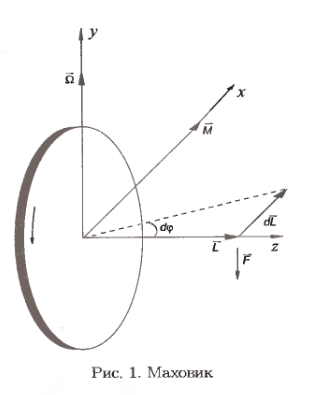
\includegraphics[width=0.40\textwidth]{img1.png}&
			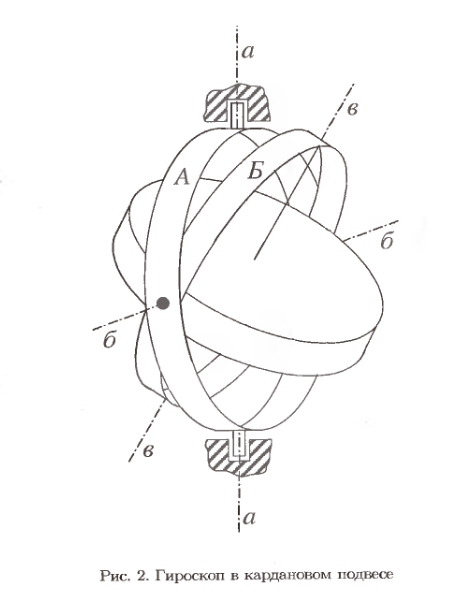
\includegraphics[width=0.40\textwidth]{img2.png}\\
		\end{array}$
	\end{center}
	
	Измерение скорости прецессии гироскопа позволяет вычислить угловую скорость вращения его ротора. Расчет производится по формуле:
	
	\begin{equation}
		\Omega = \frac{mgl}{I_z\omega_0},
	\end{equation}
	
	где $m$ -- масса груза, $l$ -- расстояние от центра карданова подвеса до точки крепления груза на оси гироскопа, $I_z$ -- момент инерции гироскопа по его главной оси вращения. $\omega_0$ -- частота его вращения относительно главной оси, $\Omega$ -- частота прецессии.\\
	Момент инерции ротора относительно оси симметрии $I_0$ измеряется по крутильным колебаниям точной копии ротора, подвешиваемой вдоль оси симметрии на десткой проволоке. Период крутильных колебаний $T_0$ зависит от момента инерции $I_0$ и модуля кручения проволоки $f$:
	
	\begin{equation}
		T_0 = 2\pi\sqrt{\frac{I_0}{f}}.
	\end{equation}
	
	Чтобы исключить модуль кручения проволоки, вместо ротора гироскопа к той же проволоке подвешивают цилиндр правильной формы с известными размерами и массой, для которого легко можно вычислить момент инерции $I_\text{ц}$. Для определения момента инерции ротора гироскопа имеем:
	
	\begin{equation}
		I_0 = I_\text{ц}\frac{T_0^2}{T_\text{ц}^2},
		\label{moment}
	\end{equation}
	Здесь $T_\text{ц}$ -- период крутильных колебаний цилиндра.\\
	\begin{center}
		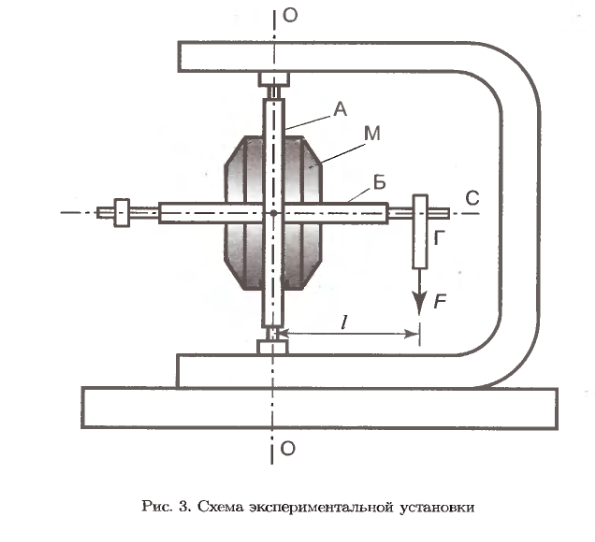
\includegraphics[width=0.8\textwidth]{img3.png}
	\end{center}
	
	Скорость вращения ротора гироскопа можно определить и не прибегая к исследованию прецессии. У используемых в работе гироскопов статор имеет две обмотки, необходимые для быстрой раскрутки гироскопа. В данной работе одну обмотку искользубт для раскрутки гироскопа, а вторую -- для измерения числа оборотов ротора. Ротор электромотора всегда немного намагничен. Вращаясь, он наводит во второй обмотке переменную ЭДС индукции, частота которой равна частоте врещения ротора. Частоту этой ЭДС можно, в частности, измерить по фигурам Лиссажу, получаемым на экране осциллографа, если на один вход подать исследуемую ЭДС, а на другой -- переменное напряжение с хорошо прокалиброванного генератора. При совпадении частот на эеране получаем эллипс.

\section{Приборы и данные}
\begin{itemize}
    \item Штангенциркуль, погрешность $\sigma_{sht} = 0,1 $ мм
    \item Секундомер, погрешность $\sigma_{sec} = 0,1 $ с (с учетом реакции экспериментатора)
    \item Осциллограф
    \item Генератор частот
    \item Весы, погрешность $\sigma_{sht} = 0,01$ г
\end{itemize}

\begin{table}[!h]
\begin{center}
\begin{tabular}{|l|l|l|l|}
\hline
        & Масса, г & Радиус, см & Период, с \\ \hline
Цилиндр & 1616,6   & 3,9        & 3,91      \\ \hline
Ротор   & 1083     & 3,4        & 3,22      \\ \hline
\end{tabular}
\caption{Данные полученные для расчета момента инерции ротора с помощью цилиндра}
\end{center}
\end{table}

\begin{table}[!h]
\begin{center}
\begin{tabular}{|l|l|l|l|}
\hline
   & Масса груза, г & Время прецессии, с & Угол поворота, рад \\ \hline
№1 & 57             & 153                & 5,76               \\ \hline
№2 & 173            & 156                & 16,76              \\ \hline
№3 & 215            & 154                & 18,85              \\ \hline
№4 & 268            & 156                & 26,44              \\ \hline
№5 & 338            & 155                & 37,7               \\ \hline
\end{tabular}
\caption{Данные для измерения прецессии, зависимость угла поворота от момента сил}
\end{center}
\end{table}

\begin{table}[!h]
\begin{center}
\begin{tabular}{|c|c|}
\hline
Плечо от груза до ц.м., мм    & 121   \\ \hline
Частота для фигур Лиссажу, Гц & 388,4 \\ \hline
\end{tabular}
\caption{Дополнительные данные}
\end{center}
\end{table}

\section{Обработка результатов}

\subsection{Нахождение момента инерции ротора}

Используя данные таблицы 1 и формулу \label{moment} получаем:
\[I_{\text{ц}} = \frac{m_{\text{ц}}R^2}{2} = (123 \pm 1,23) \cdot 10^{-5} \text{ кг}\cdot\text{м}^2 (\varepsilon_{I_{\text{ц}}} = 1\%)\]
\[I_{0} = I_{\text{ц}} \cdot \frac{T_{0}^2}{T_{\text{ц}}^2} = (8,34 \pm 0,067) \cdot 10^{-4} \text{ кг}\cdot\text{м}^2 (\varepsilon_{I_{0}} = 0,8\%)\]

\subsection{Измерение угловой скорости регулярной прецессии}

По таблице 2:
Используя формулу $\Omega = \frac{\Delta\phi}{T}$ находим угловую скорость рецессии. Далее найдем момент силы $M = mgl$ для каждой массы и $\omega = \frac{\Delta\phi^{'}}{T}, \phi = 0,17 \text{ рад}$ - угловую скорость опускания рычага.

Погрешность:
\[\sigma_{\text{случ}} = \sqrt{\frac{1}{5 \cdot 4}\sum\limits_{i=1}^{5} (\overline{\Omega_{i}} - \Omega_{i})^2}\]
\[\sigma_{\text{сист}} = \Omega \cdot \varepsilon_{T}\]
\[\sigma_{\text{полн}} = \sqrt{\sigma_{\text{случ}}^2 + \sigma_{\text{сист}}^2}\]

\begin{table}[!h]
\begin{tabular}{|c|c|c|c|c|}
\hline
   & Масса груза, $m$, г & Угловая скорость рецессии, $\Omega$, $c{^-1}$ & Момент силы, $M$, Н $\cdot$ м & Угловая скорость, $\omega$, $c^{-1}$ \\ \hline
№1 & 57                  & 0,0378 $\pm$ 0,00012                                     & 0,069                                      & 0,00110                            \\ \hline
№2 & 173                 & 0,107  $\pm$ 0,0003                                   & 0,21                                       & 0,00109                            \\ \hline
№3 & 215                 & 0,122  $\pm$ 0,0004                                     & 0,26                                       & 0,00110                            \\ \hline
№4 & 268                 & 0,17  $\pm$ 0,00055                                      & 0,324                                      & 0,00108                            \\ \hline
№5 & 338                 & 0,243 $\pm$ 0,0008                                      & 0,41                                       & 0,00111                            \\ \hline
\end{tabular}
\caption{Полученные величины $\Omega, M, \omega$}
\end{table}
\newpage
\subsection{Построение графика зависимости угловой скорости рецессии от момента силы}
С помощью расчетов из таблицы 4 построим график $\Omega(M)$
\begin{figure}[h!]
    \centering
    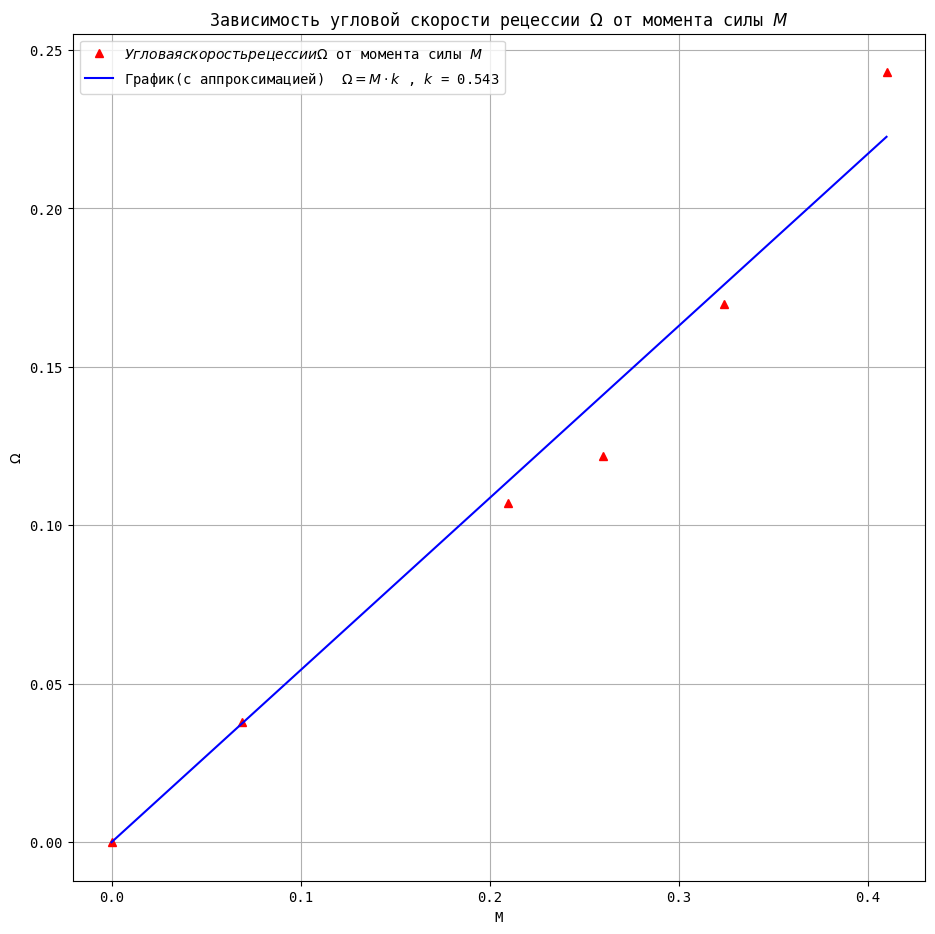
\includegraphics[width=1\textwidth]{graphic}
    \caption{График зависимости угловой скорости рецессии $\Omega$ от момента силы $M$}
\end{figure}

\subsection{Нахождение частоты вращения ротора гироскопа}

Частота вращения будет равна $\omega_{0} = \frac{1}{kI_{0}}$, где $k$ - угол наклона прямой графика $\Omega(M)$
\[k=\frac{\langle xy\rangle-\langle x\rangle \langle y\rangle}{\langle x^2\rangle - \langle x\rangle^2}\approx 0,543\]

Получаем $\omega_{0} = 2245,4 \text{ с}^{-1}$

Погрешность $\sigma_{\omega_{0}} = \omega_{0} \cdot \varepsilon_{I_{0}} \approx 17,96 \text{ с}^{-1} (\varepsilon_{\omega_{0}} = 0,8\%)$

Отсюда частота вращения ротора гироскопа будет расчитываться как $\nu = \frac{\omega_{0}}{2\pi} \approx 357,4 \text{ Гц}$

Погрешность частоты: $\sigma_{\nu} = \nu \cdot \varepsilon_{\omega_{0}} \approx 2,86 \text{ Гц}(\varepsilon_{\nu} = 0,8\%) $

Получаем частота вращения ротора гироскопа $\nu = 357,4 \pm 2,86 \text{ Гц}$ с точностью 0,8 \%.

\subsection{Определение частоты вращения по фигурам Лиссажу}
С помощью осциллографа и генератора частот подключенных к гироскопу была найдена частота вращения ротора гироскопа.

Подобранная частота $\nu = 388,4 \pm 0,5 \text{ Гц }$, при которой эллипс отображаемый на осциллографе стал неподвижным. 

Также были замечены помехи от внутренней ЭДС гироскопа, поэтому наблюдение фигуры Лиссажу было во время выключения гироскопа.

\section{Выводы}

В данной работе были полученны частоты вращения ротора гироскопа двумя способами с разными погрешностями:
\begin{itemize}
    \item Через прецессию гироскопа: $\nu_{1} = 357,4 \pm 2,86 \text{ Гц}$ с точностью 0,8 \%.
    \item Через фигуры Лиссажу:      $\nu_{2} = 388,4 \pm 0,5 \text{  Гц }$ с точностью 0,1 \%
\end{itemize}

Сравнивая результаты приходим к выводу что при расчете 1 способом на значения оказывает влияние погрешность в отличии от способа 2 где используются более точные приборы.

В работе была исследована вынужденная перцессия гироскопа, установлена зависимость скорости прецессии от момента сил действующих на ось гироскопа, и также были посчитаны частоты вращения двумя методами, а затем было проведено их сравнение с учетом погрешностей.

\end{document}
